\chapter{Thin strip graphs}
\label{chap:thinDef}

\begin{fquote}[Alan Turing][The Imitation Game]
  Sometimes it is the people no one imagines anything of who do the things that no one can imagine.
\end{fquote}

The goal of this chapter is to introduce the main subject of this thesis which is a class of graphs that lie between unit disk graphs
and mixed interval graphs called \emph{\index{thin strip graphs}}. We can define formally a \emph{\index{$c$-strip graph}} as a unit disk graph such that the centers of the disks belong to $\{(x,y) : -\infty < x < \infty, 0 \leq y \leq c\}$, more intuitively we can see this as a unit disk graph where the centers of the disks lie between two parallel horizontal lines with a distance of $c$ between them. We denote this class by SG($c$). We then have that SG($0$) = UIG and SG($\infty$) = UDG.

The definition and main work for this class comes from Breu in his thesis \cite{breuAlgorithmicAspectsConstrained1996}. However, Hayashi \textit{et al.} \cite{hayashiThinStripGraphs2017} expanded his work by defining the class of thin strip graphs. A first review of unit disk graphs will be done in the first section of this chapter, based on the original paper of Clark \textit{et al.} \cite{CLARK1990165} where unit disks graphs were defined with some interesting results.

\begin{figure}
\centering

\begin{scaletikzpicturetowidth}{\textwidth}
\begin{tikzpicture}[scale=1.5, rotate=-65]


\node[inner sep=0pt] (b) at (1,2)
    {\includegraphics[width=.1\textwidth]{res/antenna}};
\node[inner sep=0pt] (c) at (2,3)
    {\includegraphics[width=.1\textwidth]{res/antenna}};
\node[inner sep=0pt] (d) at (0,0)
    {\includegraphics[width=.1\textwidth]{res/antenna}};
\node[inner sep=0pt] (e) at (-0.5,1.5)
    {\includegraphics[width=.1\textwidth]{res/antenna}};
\node[inner sep=0pt] (e) at (0.25,3.25)
    {\includegraphics[width=.1\textwidth]{res/antenna}};


\draw[color=green]  (-0.5,1.5) circle [radius=1];
\draw[color=red]  (1,2) circle [radius=1];
\draw[color=green]  (2,3) circle [radius=1];
\draw[color=red]  (0,0) circle [radius=1];
\draw[color=blue]  (0.25,3.25) circle [radius=1];

\end{tikzpicture}
\end{scaletikzpicturetowidth}
\caption{A broadcast network with its respective unit disk graph model. The color of each disk represents the frequency of the signals sent by its broadcast node. It has to be different for adjacent antennas to avoid signal interference. The broadcast problem is equivalent to the coloring problem of the graph.}
\label{fig:antenna}
\end{figure}

\section{Unit disk graphs}

An \emph{\index{unit disk graph}} is an intersection graph of equal-sized disks on a plane - also called \emph{unitary}. The main interest of this class of graphs is its application. They can be used to create a graph-theoretic model for any kind broadcast networks. This can be useful in the case where a broadcast node needs to have a different frequency from another broadcast node that is close enough. With the unit disk graph model, we can solve this problem using algorithms for well known graph-theoretic problems such that the coloration problem.

The most studied problem for this class of graphs is its recognition and characterization. It has been proven that its recognition problem is \index{$\exists\mathbb{R}$-complete} \cite{Schaefer2013}. On the other hand, its characterization is still not complete and is an open question. Atminas \textit{et al.} tackled this problem by finding forbidden subgraphs to some of its subclasses \cite{atminasForbiddenInducedSubgraphs2016}. However, from its definition, we know that some graph-theoretic problems have different complexity when applied to unit disk graphs like the CLIQUE problem which has been proven to be polynomial when applied to UDGs \cite{CLARK1990165}. The approximation complexity of these problems has also been studied \cite{DBLP:journals/corr/abs-1712-05010}.


\section{Thin strip graphs}

A thin strip graph can be intuitively defined as a $c$-strip graph where $c$ is an arbitrarily little $\varepsilon$. Also, we can see that SG($k$) $\subseteq$ SG($l$) with $k<l$. A more strict definition emerges from this observation:

\begin{defn}
  Thin strip graphs are defined as TSG $= \bigcap_{c > 0}$ SG($c$).
\end{defn}

\begin{remark}
  SG($0$) $\neq$ TSG. We can construct a $K_{1,3}$ such that we have 3 vertices with the coordinates
  $(1,0)$, $(0,0)$, $(1,0)$ and a last one $(0,\varepsilon)$ with $\varepsilon > 0$ and arbitrarily small
  as seen in Figure \ref{fig:thinK13}.
\end{remark}

% Figure about the K_1,3 construction
\begin{figure}
\centering

\begin{scaletikzpicturetowidth}{\textwidth}
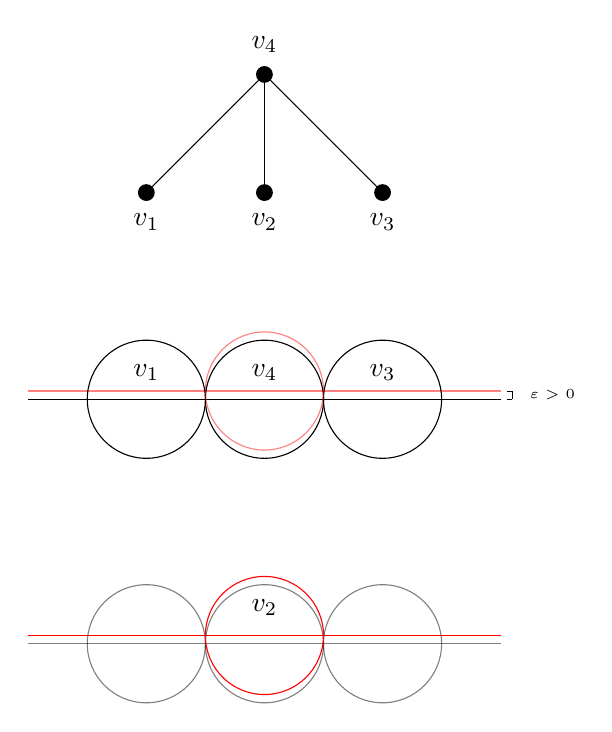
\begin{tikzpicture}[scale=1.5]

\draw (-2,0) -- (2,0);
\draw[red ,opacity = 0.5] (-2,0.07) -- (2,0.07);
\draw  (-1,0) circle [radius=0.5];
\draw[color=black] (-1,0.2265) node {$v_1$};
\draw  (0,0) circle [radius=0.5];
\draw[color=black] (0,0.2265) node {$v_4$};
\draw  (1,0) circle [radius=0.5];
\draw[color=black] (1,0.2265) node {$v_3$};

\draw[red, opacity = 0.5] (0,0.07) circle [radius=0.5];
\draw[color=black] (2.4386,0.0367) node {\tiny $\varepsilon > 0$};

% lines to describe distance (epsilon)
\draw[very thin] (2.1,0.07) -- (2.1,0);
\draw[very thin] (2.05,0.07) -- (2.1,0.07);
\draw[very thin] (2.05,0) -- (2.1,0);

\draw[opacity = 0.5] (-2,-2.07) -- (2,-2.07);
\draw[red] (-2,-2) -- (2,-2);
\draw[opacity = 0.5]  (0,-2.07) circle [radius=0.5];
\draw[opacity = 0.5]  (1,-2.07) circle [radius=0.5];
\draw[opacity = 0.5]  (-1,-2.07) circle [radius=0.5];
\draw[red] (0,-2) circle [radius=0.5];
\draw[color=black] (0,-1.765) node {$v_2$};

\node[draw,circle,inner sep=2pt,fill,label distance=1cm] (v1) at (0,2.75) {};
\draw[color=black] (0,3) node {$v_4$};
\node[draw,circle,inner sep=2pt,fill,label distance=1cm] (v3) at (0,1.75) {};
\draw[color=black] (0,1.5) node {$v_2$};
\node[draw,circle,inner sep=2pt,fill,label distance=1cm] (v2) at (-1,1.75) {};
\draw[color=black] (1,1.5) node {$v_3$};
\node[draw,circle,inner sep=2pt,fill,label distance=1cm] (v4) at (1,1.75) {};
\draw[color=black] (-1,1.5) node {$v_1$};
\draw  (v1) edge (v2);
\draw  (v1) edge (v3);
\draw  (v1) edge (v4);
\end{tikzpicture}
\end{scaletikzpicturetowidth}
\caption{A construction of $K_{1,3}$ with a disk realization, being this graph a TSG.}
\label{fig:thinK13}
\end{figure}

Two important properties about this class of graphs have been proven by Hayashi \textit{et al.} \cite{hayashiThinStripGraphs2017} which impedes us to analyse it as a case of $c$-strip graphs. We proceed to prove this properties in this section. Before that, we have to clarify an observation from the definition.

\begin{obs}
  For a realization $\phi$ of a unit disk graph $G$, $\text{diam}(\phi) \leqslant \text{diam}(G)$.
\end{obs}

This simple observation will allow us to state our first claim, which characterizes partly TSG.

\begin{claim}
  If $c^2 + \Big(\frac{\text{diam}(G)}{\alpha(G) - 1}\Big)^2 \leqslant 1$, then there is no $c$-realization of $G$.
\end{claim}

\proof{
Suppose that there exists $\phi$ a $c$-realization of $G$ such that $c^2 + \Big(\frac{\text{diam}(G)}{\alpha(G) - 1}\Big)^2 \leqslant 1$. Consider the minimum axis-parallel rectangle that covers $\phi$, and partition that rectangle into $\alpha(G) - 1$ vertical blocks of the same length. By the previous observation, the horizontal length of each block is at most of $\frac{\text{diam}(G)}{\alpha(G)-1}$. The vertical length is at most $c$. The diagonal length is then $\sqrt{c^2 + \Big(\frac{\text{diam}(G)}{\alpha(G)-1}\Big)^2} \leq 1$. This means that two points in a block are adjacent. By the pidgeonhole principile, there are two vertices of the maximum independent set on the same block, which is a contradiction. \qed
}

From this claim follows the next corollary.

\begin{figure}
\begin{center}
  \begin{scaletikzpicturetowidth}{\textwidth}
  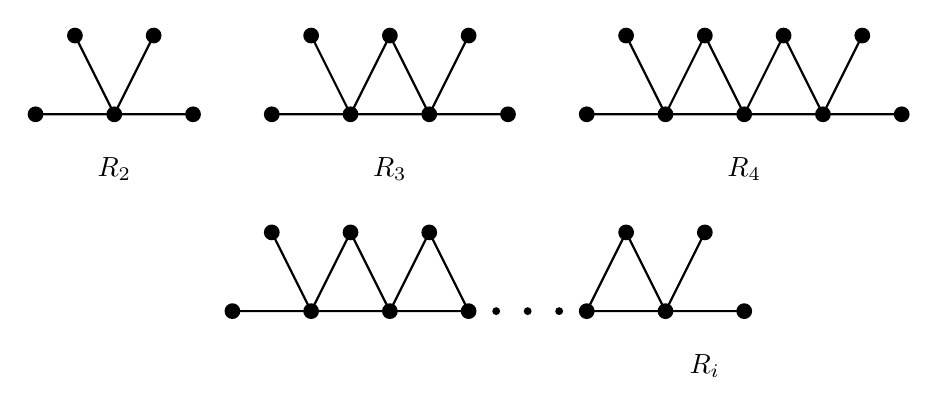
\begin{tikzpicture}[scale=1]
\def\ver{0.1} %size of a vertex
\def\x{1}

\def\xa{0.5}
\def\ya{0}

\def\xb{4}
\def\yb{0}

\def\xc{8}
\def\yc{0}

\def\xd{3.5}
\def\yd{-2.5}


%graph R_0
\path[fill] (\xa+0.5,\ya) circle (\ver);
\path[fill] (\xa+1,\ya+1) circle (\ver);
\path[fill] (\xa+2,\ya+1) circle (\ver);
\path[fill] (\xa+2.5,\ya) circle (\ver);
\path[fill] (\xa+1.5,\ya) circle (\ver);

\draw[thick] (\xa+0.5,\ya)--(\xa+1.5,\ya)--(\xa+1,\ya+1)
(\xa+2,\ya+1)--(\xa+1.5,\ya)--(\xa+2.5,\ya);

\node (1) at (\xa+1.5,\ya-0.7) {$R_2$};

%graph R_1
\path[fill] (\xb,\yb) circle (\ver);
\path[fill] (\xb+1,\yb) circle (\ver);
\path[fill] (\xb+2,\yb) circle (\ver);
\path[fill] (\xb+3,\yb) circle (\ver);
\path[fill] (\xb+0.5,\yb+1) circle (\ver);
\path[fill] (\xb+1.5,\yb+1) circle (\ver);
\path[fill] (\xb+2.5,\yb+1) circle (\ver);

\draw[thick] (\xb,\yb)--(\xb+1,\yb)--(\xb+2,\yb)--(\xb+3,\yb)
(\xb+0.5,\yb+1)--(\xb+1,\yb)--(\xb+1.5,\yb+1)--(\xb+2,\yb)--(\xb+2.5,\yb+1);

\node (1) at (\xb+1.5,\yb-0.7) {$R_3$};


%graph R_2
\path[fill] (\xc,\yc) circle (\ver);
\path[fill] (\xc+1,\yc) circle (\ver);
\path[fill] (\xc+2,\yc) circle (\ver);
\path[fill] (\xc+3,\yc) circle (\ver);
\path[fill] (\xc+4,\yc) circle (\ver);
\path[fill] (\xc+0.5,\yc+1) circle (\ver);
\path[fill] (\xc+1.5,\yc+1) circle (\ver);
\path[fill] (\xc+2.5,\yc+1) circle (\ver);
\path[fill] (\xc+3.5,\yc+1) circle (\ver);

\draw[thick] (\xc,\yc)--(\xc+1,\yc)--(\xc+2,\yc)--(\xc+3,\yc)--(\xc+4,\yc)
(\xc+0.5,\yc+1)--(\xc+1,\yc)--(\xc+1.5,\yc+1)--(\xc+2,\yc)--(\xc+2.5,\yc+1)--(\xc+3,\yc)--(\xc+3.5,\yc+1);

\node (1) at (\xc+2,\yc-0.7) {$R_4$};

%graph R_i
\path[fill] (\xd,\yd) circle (\ver);
\path[fill] (\xd+1,\yd) circle (\ver);
\path[fill] (\xd+2,\yd) circle (\ver);
\path[fill] (\xd+3,\yd) circle (\ver);
\path[fill] (\xd+4.5,\yd) circle (\ver);
\path[fill] (\xd+5.5,\yd) circle (\ver);
\path[fill] (\xd+6.5,\yd) circle (\ver);
\path[fill] (\xd+0.5,\yd+1) circle (\ver);
\path[fill] (\xd+1.5,\yd+1) circle (\ver);
\path[fill] (\xd+2.5,\yd+1) circle (\ver);
\path[fill] (\xd+5,\yd+1) circle (\ver);
\path[fill] (\xd+6,\yd+1) circle (\ver);

\fill (\xd+3.35,\yd) circle (\ver/2);
\fill (\xd+3.75,\yd) circle (\ver/2);
\fill (\xd+4.15,\yd) circle (\ver/2);

\draw[thick] (\xd,\yd)--(\xd+3,\yd)
(\xd+4.5,\yd)--(\xd+6.5,\yd)
(\xd+0.5,\yd+1)--(\xd+1,\yd)--(\xd+1.5,\yd+1)--(\xd+2,\yd)--(\xd+2.5,\yd+1)--(\xd+3,\yd)
(\xd+4.5,\yd)--(\xd+5,\yd+1)--(\xd+5.5,\yd)--(\xd+6,\yd+1);


\node (1) at (\xd+6,\yd-0.7) {$R_i$};

\end{tikzpicture}
\end{scaletikzpicturetowidth}
\end{center}
\caption{The class $\mathcal{R}$, with the indexes arranged for the thin strip graph theorem. \cite{joosCharacterizationMixedUnit2013}}\label{fig:graphsR'}
\end{figure}

\begin{corollary}
  If $\text{diam}(G) < \alpha(G) - 1$, then $G \notin \text{SG}\Bigg(\sqrt{1 - \Big(\frac{\text{diam}(G)}{\alpha(G)-1}\Big)^2}\Bigg)$.
\end{corollary}

Now we are going to prove the main property of TSG. For that, we are going to use the family of graphs $\mathcal{R}$ as seen in Figure \ref{fig:graphsR} of the past chapter. For this proof, we are going to rename it and change the indexes of the graphs as shown in Figure \ref{fig:graphsR'}. Let $\Gamma(G) = \sqrt{1 - \Big(\frac{\text{diam}(G)}{\alpha(G)-1}\Big)^2}$ for simplicity and $\gamma(i) = \sqrt{1 - \Big(\frac{i}{i+1}\Big)^2}$. The proof of the theorem will follow the next lemmas, where we show that $\mathcal{R}$ is indeed a forbidden family of subgraphs of TSG.

\begin{lemma}
  For each $k \geqslant 2$, $R_k$ has no $\gamma(k)$-realization.
\end{lemma}

\proof{
  Effectively, $\text{diam}(R_k) = k$ and $\alpha(R_k) \geqslant k + 2$, $\Gamma(R_k) = \gamma(k)$ holds. The lemma follows from the previous corollary. \qed
}

\begin{lemma}
  For each odd integer $k \geqslant 3$, $R_k$ has a $(\gamma(k) + \varepsilon)$-realization with $\varepsilon > 0$.
\end{lemma}

\proof{See \cite{hayashiThinStripGraphs2017}.}

And because $\lim_{k \to \infty}\gamma(k) = 0$, the next theorem follows.

\begin{theorem}[Hayashi et al. \cite{hayashiThinStripGraphs2017}]
  There is no constant $t$ such that SG($t$) = TSG.
\end{theorem}

Also, a corollary is presented.

\begin{theorem}[Hayashi et al. \cite{hayashiThinStripGraphs2017}]
  There is no constant $t$ such that SG($t$) = UDG.
\end{theorem}

\proof{

Suppose that there exists a constant $t$ such that SG($t$) = UDG. Let $G_k$ be a $k \times k$ grid with $k \geqslant 16t$. We have that $G_k \in UDG$. Let $\phi_k$ be a $t$-realization of $G_k$. By the first observation of this section, all the centers of disks lie in a rectangle $R$ of side lengths $t$ and $\text{diam}(G_k) < 2k$, If $\alpha(G_k) \geqslant \frac{k^2}{2}$, there must be at least $\frac{k^2}{2}$ points such that there is a distance of at least $1$ between them. On the other hand, we can cover $R$ by at most $\Bigl\lceil \frac{t}{\sqrt{\frac{1}{2}}}\Bigr\rceil \Bigl\lceil \frac{2k}{\sqrt{\frac{1}{2}}}\Bigr\rceil < 8tk < \frac{k^2}{2}$ squares of diagonal length 1. By the pidgeonhole principle, there is a square with two points of the maximum independent set of $G_k$.

}

Hayashi \textit{et al.} left some open problems. We try to elaborate the knowledge around some of these problems
to understand them better, mainly for the recognition of this class of graphs. Before that, we see where this class lies in the hierarchy of classes. We know by definition that TSG $\subsetneq$ UDG.

\subsection{Interval graphs}

Thin strip graphs share their geometrical structure with interval graphs (remember SG($0$) = UIG). In this subsection, we overview the results of Hayashi et al. \cite{hayashiThinStripGraphs2017} where they find maximal and minimal superclasses for TSG in the interval graphs presented in chapter \ref{chap:interval}. The following theorem will be proven by taking the proof written by Hayashi \textit{et al.} in order to use their mapping in other theorems.

\begin{theorem}[Hayashi et al. \cite{hayashiThinStripGraphs2017}]
  \label{theo:muigTSG}
  MUIG $\subsetneq$ TSG.
\end{theorem}

\proof{
First, we prove that MUIG $\neq$ TSG. This can be proven because $C_4 \in$ TSG if we take as points $(0,0),(0,\varepsilon),(1,0),(1,\varepsilon)$ with $1 >\varepsilon > 0$ and $C_4 \notin$ MUIG because it is a chordal graph.

Then, we have to prove that MUIG $\subseteq$ TSG. Let $G = (V,E) \in$ MUIG where each vertex is a unit mixed interval denoted as $I_v$. We define $t = \min\{|I_u\cap I_v| : |I_u\cap I_v| > 0, \{I_u,I_v\} \subseteq V\}$ and $s = \min\{\ell(I_v) - r(I_u) : \ell(I_v) > r(I_u), \{I_u,I_v\} \subseteq V\}$. We have then $t$ being the minimum length of an intersection bigger than zero (that is, not endpoint-adjacent) and $s$ is the minimum distance between non-adjacent vertices (also not endpoint-adjacent). We also define $c(I_v) = \frac{\ell(I_v) + r(I_v)}{2}$ as the center of the interval and $p(I_v) = (-1)^{\left \lfloor{c(I_v)}\right \rfloor }$.

Let $d$ be a real such that $0 < d < \frac{2}{3}$, $d\leq \frac{t}{4}$, $d < \frac{s}{2}$ and $\varepsilon \geq 2\sqrt{d-d^2}$. If we let $h = \sqrt{d-d^2}$, then we can create a $2h$-realization of $G$ with the following mapping:

\[ \phi(v) =
  \begin{cases}
      (c(I_v),0) & \text{if}\  I_v\  \text{is a closed interval} \\
      (c(I_v),hp(I_v)) & \text{if}\  I_v\  \text{is an open interval} \\
      (c(I_v)-d,hp(I_v)) & \text{if}\  I_v\  \text{is a closed-open interval} \\
      (c(I_v)+d,hp(I_v)) & \text{if}\  I_v\  \text{is an open-closed interval}
   \end{cases}
\]

For two vertices $u$ and $v$ of $G$ such that $u \leq v$, we have the three following cases:

\begin{enumerate}
  \item $r(I_u) < \ell(I_v)$:

    $I_u$ and $I_v$ are not adjacents, which means that $\text{dist}(\phi(u),\phi(v)) > 1$.
    If we minimize the distance between them we have $\phi(u) = (c(I_u)+d,hp(I_u))$ and $\phi(v) = (c(I_v)-d,hp(I_v))$ with $p(I_u) = p(I_v)$. Therefore, we only have to compare their $x$-coordinates:

    $$\text{dist}(\phi(u),\phi(v)) \geq (c(I_v)-d) - (c(I_u)+d) = c(I_v)-c(I_u) - 2d$$

    By definition, $s \leq l(I_v)-r(I_u)$. If we take the centers, then $s \leq c(I_v)-c(I_u) -1$, which means finally that $s +1 \leq c(I_v)-c(I_u)$

    $$\text{dist}(\phi(u),\phi(v)) \geq s + 1 - 2d > 1$$

  \item $r(I_u) > \ell(I_v)$:
    In this case $u$ and $v$ are adjacent. We maximize $\text{dist}(\phi(u),\phi(v))$ when $\phi(u) = (c(I_u)-d,hp(I_u))$ and $\phi(v) = (c(I_v)+d,hp(I_v))$ with $p(I_u) \neq p(I_v)$. Therefore,

\[    \begin{split}
    \text{dist}(\phi(u),\phi(v)) & \leq \sqrt{((c(I_v)+d)-(c(I_u)-d))^2 + (h+h)^2} \\
     & \text{with the same reasoning as before}\  c(I_v)-c(I_u) \leq 1-t\\
     & \leq \sqrt{(1-t+2d)^2 + 4h^2} \\
     & \leq \sqrt{(1-4d+2d)^2 + 4(d-d^2)} \\
     & = \sqrt{1-4d+4d^2 + 4d-4d^2} = 1
    \end{split}
\]

  \item $r(I_u) = \ell(I_v)$:

  In this case, $u$ and $v$ are adjacent only if $r(I_u)$ and $I_v$ are closed. We know that $c(I_v) = c(I_u)+1$ and $p(I_u) \neq p(I_v)$. Without loss of generality, we suppose that $p(I_u) = 1$ and $p(I_v) = -1$. We have two cases:
  \begin{enumerate}
    \item Both ends are closed. So we have this set of possible assignments for each one of the vertices:

    $$\phi(u) \in \{(c(I_u),0), (c(I_u)+d,h)\}$$
    $$\phi(v) \in \{(c(I_u)+1,0), (c(I_u)+1-d,-h)\}$$
    This gives us a rectangle with its diagonal smaller than one.

\item One of the ends is closed, we suppose $r(I_u)$ is open. In this case, we have these solutions:

  $$\phi(u) \in \{(c(I_u)-d,h), (c(I_u),h)\}$$
  $$\phi(v) \in \{(c(I_u)+1,0), (c(I_u)+1,-h), (c(I_u)+1\pm d,-h)\}$$

  Every distance between every points is greater than 1 if we take into consideration the domain of $d$. \qed

  \end{enumerate}
\end{enumerate}
}

From this theorem, UIG $\subsetneq$ TSG. Actually, there exists a stronger connection between these two classes:

\begin{theorem}[Breu \cite{breuAlgorithmicAspectsConstrained1996}]
  \label{theo:induced_TSG}
  Let $G$ a $c$-strip graph with $c \in \mathbb{R}_0^+$. $G$ has an induced $K_{1,3}$ or $C_4$ if and only if $G$ is not an unit interval graph.
\end{theorem}

Thin strip graphs can also be seen as unfettered unit interval graphs, which means that if a graph is a thin strip graph, then we can partition this graph with a level structure where each level is a clique. This information will be relevant in the next section.

\begin{theorem}[Hayashi et al. \cite{hayashiThinStripGraphs2017}]
  TSG $\subsetneq$ UUIG.
\end{theorem}

\proof{
The inequality is proven by Theorem \ref{theo:uuigudg} because TSG $\subset$ UDG by definition. We only have to show that TSG $\subseteq$ UUIG. Let $G = (V,E)$ a TSG with $V = \{v_1, v_2, \dots, v_n\}$ and $n \geqslant 2$. Let $\varepsilon \leqslant \frac{\sqrt{8n+1}}{4n + 1}$ and $\phi$ the $\varepsilon$-realization of $G$. We sort the vertices from left to right, thus $0 \leqslant \phi_x(v_1) \leqslant \phi_x(v_2) \leqslant \phi_x(v_3) \leqslant \dots \leqslant \phi_x(v_n)$. Let $\delta = \min(\{\sqrt{1+\varepsilon^2} - 1\} \cup \{\text{dist}(\phi(v_i), \phi(v_j)) - 1 : \{v_i,v_j\} \notin E\})$.

Now we construct another $\varepsilon$-realization $\phi'$ that is built by moving every disk to the left as much as possible, by keeping the same $y$-coordinates and the condition of adjacency $0 \leqslant \phi'_x(v_1) \leqslant \phi'_x(v_2) \leqslant \phi'_x(v_3) \leqslant \dots \leqslant \phi'_x(v_n)$. This $\phi'$ realization can be built as an optimal solution of this program:

\begin{gather*}
\max \quad \sum_{1\leqslant i \leqslant n} x_i \\
\begin{aligned}
\textup{subject to}\quad (x_i - x_j)^2 + (\phi_y(v_i) - \phi_y(v_j))^2  &\leqslant  1\ \ \ \ \text{s.t.}\  \{v_i,v_j\} \in E\\
(x_i - x_j)^2 + (\phi_y(v_i) - \phi_y(v_j))^2  &\leqslant  1 + \delta\ \ \ \ \text{s.t.}\  \{v_i,v_j\} \notin E\\
0 \leqslant x_1 \leqslant x_2 \leqslant x_3 \leqslant \dots \leqslant x_n \\
\end{aligned}
\end{gather*}

Recall that $\phi_y(v_i)$ stays the same so they are constants in our program. If we develop the conditions of our program we find that this is a linear program and it has an optimal solution:

\begin{gather*}
\max \quad \sum_{1\leqslant i \leqslant n} x_i \\
\begin{aligned}
\textup{subject to}\quad x_i - x_j &\leqslant \sqrt{1 - (\phi_y(v_i) - \phi_y(v_j))^2}\ \ \ \ \text{s.t.}\  \{v_i,v_j\} \in E\\
x_i - x_j &\leqslant \sqrt{(1 + \delta) - (\phi_y(v_i) - \phi_y(v_j))^2}\ \ \ \ \text{s.t.}\  \{v_i,v_j\} \notin E\\
0 &\leqslant x_1 \leqslant x_2 \leqslant x_3 \leqslant \dots \leqslant x_n \\
\end{aligned}
\end{gather*}

We construct a digraph $D = (V,A)$ based on the positions of the vertices of $G$ in $\phi'$. An arc $(v_i, v_j) \in A$ if and only if:

\begin{enumerate}
  \item $i > j$, $\{v_i, v_j\} \in E$ and $\text{dist}(\phi'(v_i), \phi'(v_j)) = 1$ called \emph{left arcs}.
  \item $i < j$, $\{v_i, v_j\} \notin E$ and $\text{dist}(\phi'(v_i), \phi'(v_j)) = 1 + \delta$ called \emph{right arcs}.
  \item $i < j$ and $\phi_x'(v_i) = \phi_x'(v_j)$ called \emph{vertical arcs}.
\end{enumerate}

Based on the optimality of the linear program, we should have a path between $v_1$ and $v_i$ with $1 \leq i \leqslant n$. We can prove this in the next claim.

\begin{claim}\label{claim:D_direct}
  In $D$, there is a directed path from $v_1$ to $v_i$ for each $v_i \in V$.
\end{claim}

\begin{proof}[Proof of Claim \ref{claim:D_direct}]
  Let $S$ be a non-empty subset of $V$ and $v_1 \in V \setminus S$. Assume that there is no arc from $V \setminus S$ to $S$. That means that every vertex of $S$ can be shifted to the left to meet the condition of optimality. This contradicts the optimality of $x_i$. Therefore, there is an arc from $V\setminus S$ to $S$ for all $S \subset V$ such that $v_i \notin S$. This implies the claim.
\end{proof}

For each $k$, $P_k$ is the shortest directed path $v_1 \dots v_k$ in $D$. Let $\ell_k$ and $r_k$ be the number of left arcs and right arcs in $P_k$, respectively. Clearly, $r_k + \ell_k < n$.

\begin{claim}\label{claim:neighbours}
  For every $k$, $(r_k - \ell_k) - \frac{\sqrt{1 - \varepsilon^2}}{2} \leqslant x_k \leqslant (r_k - \ell_k) + \frac{\sqrt{1 - \varepsilon^2}}{2}$.
\end{claim}

\begin{proof}[Proof of Claim \ref{claim:neighbours}]
  With a left arc, the $x$-coordinate increases by at least $\sqrt{(1 + \delta)^2 - \varepsilon^2}$ and at most by $\sqrt{1 + \delta}$. With a left arc, it decreases by at least $\sqrt{1 - \varepsilon^2}$ and at most $1$. Clearly, vertical arcs do not change the $x$-coordinate. It holds that:

  $$r_k \sqrt{(1 + \delta)^2 - \varepsilon^2} - \ell_k \leqslant x_k \leqslant r_k(1 + \delta) - \ell_k \sqrt{1 - \varepsilon^2}$$

  which implies:

  $$(r_k - \ell_k) - r_k \Big(1 -\sqrt{(1 + \delta)^2 - \varepsilon^2}\Big) \leqslant x_k \leqslant (r_k - \ell_k) + r_k\delta + \ell_k \Big(1 - \sqrt{1 - \varepsilon^2} \Big)$$

  Which is similar to the inequality to prove. Actually, to prove the inequality of the claim we have to prove the following equations:

  \begin{equation}\label{eq:first_condition}
    r_k \Big(1 -\sqrt{(1 + \delta)^2 - \varepsilon^2}\Big) \leqslant \frac{\sqrt{1 - \varepsilon^2}}{2}
  \end{equation}

  \begin{equation}\label{eq:second_condition}
    r_k\delta + \ell_k \Big(1 - \sqrt{1 - \varepsilon^2} \Big) \leqslant \frac{\sqrt{1 - \varepsilon^2}}{2}
  \end{equation}

  By the value of $\delta$, the left side of both equations are nonnegative. We can then show only the next equation:

  \begin{equation}\label{eq:third_condition}
      r_k \Big(1 -\sqrt{(1 + \delta)^2 - \varepsilon^2}\Big) + r_k\delta + \ell_k \Big(1 - \sqrt{1 - \varepsilon^2} \Big) \leqslant \frac{\sqrt{1 - \varepsilon^2}}{2}
  \end{equation}

  If we suppose that Equation \ref{eq:third_condition} does not hold and since $n > r_k + \ell_k$:

  \begin{equation}\label{eq:fourth_condition}
      n \Big(\Big(1 -\sqrt{(1 + \delta)^2 - \varepsilon^2}\Big) + \delta + \Big(1 - \sqrt{1 - \varepsilon^2} \Big)\Big) > \frac{\sqrt{1 - \varepsilon^2}}{2}
  \end{equation}

  By developing, we show that $1 - \sqrt{(1 + \delta)^2 - \varepsilon^2} + \delta \leqslant 1 - \sqrt{1 - \varepsilon^2}$ for $0 \leqslant \varepsilon \leqslant 1$ and $\delta > 0$. Then it holds that $2n \Big(1 - \sqrt{1 - \varepsilon^2} \Big) > \frac{\sqrt{1 - \varepsilon^2}}{2}$. This implies that $\varepsilon > \frac{\sqrt{8n + 1}}{4n + 1}$, which is a contradiction. Thus, Equation \ref{eq:third_condition} is correct which proves the claim.
\end{proof}

By Claim \ref{claim:neighbours}, we can classify the vertices in levels $L_k = \{v_i : r_k - \ell_k = k\}$. By the claim we imply that if $u,w \in L_k$, then $\phi'(u)$ and $\phi'(w)$ are placed on a rectangle $\varepsilon \times \sqrt{1 - \varepsilon^2}$.
Thus, $L_k$ is a clique. Now if we take another level $k'$ such that $|k - k'| \geqslant 2$ with $v_k \in L_k$ and $v_{k'} \in L_{k'}$, then $\phi'_x(v_k) - \phi'_x(v_{k'}) \geqslant k
- k' - \sqrt{1 - \varepsilon^2} \geqslant 2 - \sqrt{1 - \varepsilon^2} > 1$, which means that for $v_k \in L_k$: $N(v_k) \subseteq L(v_{k-1}) \cup L(v_{k}) \cup L(v_{k+1})$. Thus, $G$ is an unfettered unit interval graph. \qed}


\begin{figure}
\begin{center}
\begin{scaletikzpicturetowidth}{\textwidth}
\begin{tikzpicture}[scale=1]
  \node (0) [draw, rounded rectangle] {co-comparability graphs};
  \node (1) [below= of 0, draw, rounded rectangle] {unfettered unit interval graphs};
  \node (2) [below=of 1, draw, rounded rectangle] {thin strip graphs};
  \node (3) [below=of 2, draw, rounded rectangle] {mixed unit interval graphs};
  \node (4) [below=of 3, draw, rounded rectangle] {unit interval graphs};
  \node (5) [left=of 1, draw, rounded rectangle] {unit disk graphs};
  \node (6) [left=of 2, below=of 5] {};
  \draw[<-] (0) edge (1) (1) edge (2) (2) edge (3) (3) edge (4) (5) edge (6.south);
  \draw[-] (2) edge (6.south);

\end{tikzpicture}
\end{scaletikzpicturetowidth}
\end{center}
  \caption{Extension of the graph classes diagram from Figure \ref{fig:hierarchyTSG} with \emph{TSG} and \emph{UDG}.}
\label{fig:hierarchyTSG}
\end{figure}

\section{Characterization of thin strip graphs}

One of the main goals of this thesis is to characterize thin strip graphs with forbidden induced subgraphs. We know that TSG is an hereditary class, then a way to characterize this class of graphs is by looking for its forbidden subgraphs the same way as MUIG has been characterized by Joos. Furthermore, MUIG $\subsetneq$ TSG by Theorem \ref{theo:muigTSG}, so the first we can do is to check if the forbidden subgraphs of MUIG are also for TSG.


\subsection{Mixed unit interval graph forbidden subgraphs}

In the previous section we have shown that MUIG $\subsetneq$ TSG \ref{theo:muigTSG}. Here we are going to overview these forbidden induced subgraphs and we their inclusion in TSG. Moreover, we will verify if one of these families is at least in UUIG. This will help us to add thin strip graphs to the hierarchy of classes we are building.

In this subsection, we are going to see the relationship between thin strip graphs and mixed unit interval graphs.

\begin{figure}
\begin{center}
  \begin{scaletikzpicturetowidth}{\textwidth}
  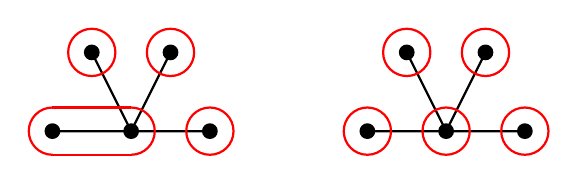
\begin{tikzpicture}[scale=1]
\def\ver{0.1} %size of a vertex
\def\x{1}

\def\xa{0.5}
\def\ya{0}

\def\xd{4.5}
\def\yd{0}


%graph R_0
\path[fill] (\xa+0.5,\ya) circle (\ver);
\path[fill] (\xa+1,\ya+1) circle (\ver);
\path[fill] (\xa+2,\ya+1) circle (\ver);
\path[fill] (\xa+2.5,\ya) circle (\ver);
\path[fill] (\xa+1.5,\ya) circle (\ver);

\draw[thick] (\xa+0.5,\ya)--(\xa+1.5,\ya)--(\xa+1,\ya+1)
(\xa+2,\ya+1)--(\xa+1.5,\ya)--(\xa+2.5,\ya);


\draw[thick,red] (\xa+2,\ya+1+ \ver+0.2) coordinate(a1)  arc (90:450:\ver +0.2) coordinate(a2);

\draw[thick,red] (\xa+1,\ya+1+ \ver+0.2) coordinate(d1)  arc (90:450:\ver +0.2) coordinate(d2);

\draw[thick,red] (\xa+2.5,\ya+ \ver+0.2) coordinate(e1)  arc (90:450:\ver +0.2) coordinate(e2);

\draw[thick,red] (\xa+0.5,\ya+ \ver+0.2) coordinate(b1)  arc (90:270:\ver +0.2) coordinate(b2);
\draw[thick,red] (\xa+1.5,\ya- \ver-0.2) coordinate(c1)  arc (270:450:\ver +0.2) coordinate(c2);

% reliate
\draw[thick,red] (c1) -- (b2) (c2)--(b1);

%graph R_0
\path[fill] (\xd+0.5,\yd) circle (\ver);
\path[fill] (\xd+1,\yd+1) circle (\ver);
\path[fill] (\xd+2,\yd+1) circle (\ver);
\path[fill] (\xd+2.5,\yd) circle (\ver);
\path[fill] (\xd+1.5,\yd) circle (\ver);

\draw[thick] (\xd+0.5,\yd)--(\xd+1.5,\yd)--(\xd+1,\yd+1)
(\xd+2,\yd+1)--(\xd+1.5,\yd)--(\xd+2.5,\yd);

\draw[thick,red] (\xd+2,\yd+1+ \ver+0.2) coordinate(a1)  arc (90:450:\ver +0.2) coordinate(a2);
\draw[thick,red] (\xd+1,\yd+1+ \ver+0.2) coordinate(d1)  arc (90:450:\ver +0.2) coordinate(d2);
\draw[thick,red] (\xd+2.5,\yd+ \ver+0.2) coordinate(e1)  arc (90:450:\ver +0.2) coordinate(e2);
\draw[thick,red] (\xd+1.5,\yd+ \ver+0.2) coordinate(d1)  arc (90:450:\ver +0.2) coordinate(d2);
\draw[thick,red] (\xd+0.5,\yd+ \ver+0.2) coordinate(e1)  arc (90:450:\ver +0.2) coordinate(e2);


\end{tikzpicture}
\end{scaletikzpicturetowidth}
\end{center}
\caption{Every possible clique partition of $R_0$. You may notice that none of the partition is a level structure.}\label{fig:R0level}
\end{figure}

\begin{figure}[H]
\begin{center}
  \begin{scaletikzpicturetowidth}{\textwidth}
  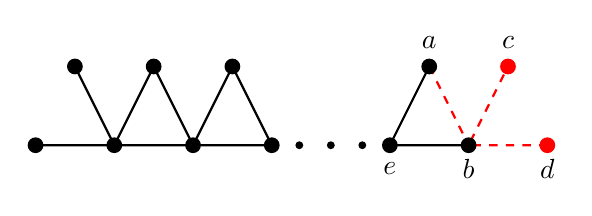
\begin{tikzpicture}[scale=1]
\def\ver{0.1} %size of a vertex
\def\x{1}

\def\xd{0}
\def\yd{0}

\draw[thick] (\xd,\yd)--(\xd+3,\yd)
(\xd+4.5,\yd)--(\xd+5.5,\yd)
(\xd+0.5,\yd+1)--(\xd+1,\yd)--(\xd+1.5,\yd+1)--(\xd+2,\yd)--(\xd+2.5,\yd+1)--(\xd+3,\yd)
(\xd+4.5,\yd)--(\xd+5,\yd+1);

\draw[thick, dashed, color=red] (\xd+6.5,\yd) -- (\xd+5.5,\yd)--(\xd+6,\yd+1) (\xd+5,\yd+1)--(\xd+5.5,\yd);

%graph R_i
\path[fill] (\xd,\yd) circle (\ver);
\path[fill] (\xd+1,\yd) circle (\ver);
\path[fill] (\xd+2,\yd) circle (\ver);
\path[fill] (\xd+3,\yd) circle (\ver);
\path[fill] (\xd+4.5,\yd) circle (\ver);
\path[fill] (\xd+5.5,\yd) circle (\ver);
\path[fill, color=red] (\xd+6.5,\yd) circle (\ver);
\path[fill] (\xd+0.5,\yd+1) circle (\ver);
\path[fill] (\xd+1.5,\yd+1) circle (\ver);
\path[fill] (\xd+2.5,\yd+1) circle (\ver);
\path[fill] (\xd+5,\yd+1) circle (\ver);
\path[fill, color=red] (\xd+6,\yd+1) circle (\ver);

\fill (\xd+3.35,\yd) circle (\ver/2);
\fill (\xd+3.75,\yd) circle (\ver/2);
\fill (\xd+4.15,\yd) circle (\ver/2);

\node (1) at (\xd+5.5,\yd-0.3) {$b$};
\node (2) at (\xd+6.5,\yd-0.3) {$d$};
\node (2) at (\xd+4.5,\yd-0.3) {$e$};
\node (4) at (\xd+5,\yd+1+0.3) {$a$};
\node (3) at (\xd+6,\yd+1+0.3) {$c$};

\end{tikzpicture}
\end{scaletikzpicturetowidth}
\end{center}
\caption{The graph $R_{i+1}$. You can see that the red edges and vertices are what differ from $R_i$.}\label{fig:ri+1}
\end{figure}

\begin{theorem}[Hayashi et al. \cite{hayashiThinStripGraphs2017}]
  $\mathcal{R}$ is a forbidden induced subgraph family of UUIG.
\end{theorem}

\begin{proof}
  We can prove this by induction on $i$.

  \begin{itemize}
    \item \emph{Case $i=0$}: $R_0 \notin$ UUIG because there is no clique partition of $R_0$ that is also a level structure as seen in Figure \ref{fig:R0level}.
    \item \emph{Case $i = i+1$}: We suppose that every valid clique partition of $R_i$ is not a level structure. See in Figure \ref{fig:ri+1} the edges and vertices that we add to generate $R_{i+1}$. We call $a,b$ the vertices that were disjoint in $R_i$ and $c,d$ the new vertices. These two vertices are adjacent to $b$.

    Let $\{b,c\}$ or $\{b,d\}$ be a level of our clique partition. By the hypothesis of induction we know that this is partition is not a level structure because this partition is a valid partition of $R_i$ because $a$ and $b$ are in different levels. The only way to create a new partition that is not a valid clique partition of $R_i$ is if $\{a,b\}$ is a level. In this case, however, the clique level $\{a,b\}$ will be adjacent to three cliques $\{c\}, \{d\}$ and $\{e, \dots\}$ so this clique partition is not a level structure either.
  \end{itemize}

  This proves that $R_i$ for every $i \in \mathbb{N}_0$ has not a clique level structure; thus, it is not an UUIG.
\end{proof}

We see that $\mathcal{R}$ is a family of forbidden subgraphs of TSG. Nevertheless, the rest of the forbidden subgraphs for MUIG are thin strip graphs. The main reason is because they are unfettered unit interval graphs. We see our first example with the forbidden graph for MUIG $F$.

\begin{figure}
\begin{center}
  \begin{scaletikzpicturetowidth}{\textwidth}
  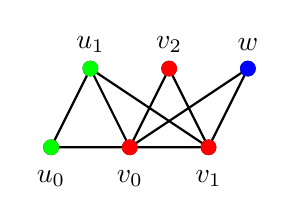
\begin{tikzpicture}[scale=1]
    \def\ver{0.1} %size of a vertex
    \def\x{1}

    \def\xa{0}
    \def\ya{0}

    %G_1
    \path[fill] (\xa+1,\ya) circle (\ver);
    \path[fill] (\xa+2,\ya) circle (\ver);
    \path[fill] (\xa+0.5,\ya+1) circle (\ver);
    \path[fill] (\xa+1.5,\ya+1) circle (\ver);
    \path[fill] (\xa+2.5,\ya+1) circle (\ver);
    \path[fill] (\xa,\ya) circle (\ver);

    \draw[thick] (\xa+1,\ya)--(\xa+2,\ya)
    (\xa+1,\ya)--(\xa+0.5,\ya+1)--(\xa+2,\ya)
    (\xa+1,\ya)--(\xa+2.5,\ya+1)--(\xa+2,\ya)
    (\xa+1,\ya)--(\xa+1.5,\ya+1)--(\xa+2,\ya)
    (\xa+1,\ya)--(\xa,\ya)--(\xa+0.5,\ya+1);

    \path[fill=red] (\xa+1,\ya) circle (\ver);
    \path[fill=red] (\xa+2,\ya) circle (\ver);
    \path[fill=green] (\xa+0.5,\ya+1) circle (\ver);
    \path[fill=red] (\xa+1.5,\ya+1) circle (\ver);
    \path[fill=blue] (\xa+2.5,\ya+1) circle (\ver);
    \path[fill=green] (\xa,\ya) circle (\ver);

    \node (1) at (\xa,\ya-0.4) {$u_0$};
    \node (1) at (\xa+0.5,\ya+1.3) {$u_1$};
    \node (1) at (\xa+1,\ya-0.4) {$v_0$};
    \node (1) at (\xa+2,\ya-0.4) {$v_1$};
    \node (1) at (\xa+1.5,\ya+1.3) {$v_2$};
    \node (1) at (\xa+2.5,\ya+1.3) {$w$};

\end{tikzpicture}
\end{scaletikzpicturetowidth}
\end{center}
\caption{The graph $F$ where each level is represented by a different color.}\label{fig:graphF_clique}
\end{figure}

\begin{figure}[b]
\begin{center}
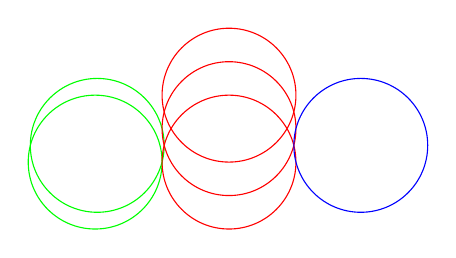
\begin{tikzpicture}[scale=1.7]

\def\ver{0.5}
\def\verp{0.04} %size of a vertex
\def\epsilon{0.5}


\draw[color=green] ({((\epsilon/4)*(\epsilon/4) - 1)*2*\ver},{(\epsilon/4)*2*\ver}) circle (\ver);
\draw[color=green] (-1,0) circle (\ver);

\draw[color=red] (0,0) circle (\ver);
\draw[color=red] (0,{(\epsilon / 2) *2* \ver}) circle (\ver);
\draw[color=red] (0,{(2* \epsilon / 2)*2* \ver}) circle (\ver);

\draw[color=blue] ({(1 - (\epsilon/4)*(\epsilon/4))*2*\ver},{(\epsilon/4)*2*\ver}) circle (\ver);


\end{tikzpicture}
\end{center}
\caption{Realization of $F$ as a thin strip graph.}\label{fig:graphF_thin}
\end{figure}

\begin{theorem}
  $F \in$ TSG.
\end{theorem}

\proof{
To prove this we have to find an $\varepsilon$-realization for our graph $F = (V,E)$ with $\varepsilon$ arbitrarily small. Let $\phi(v)$ be the mapping of our vertices on the plane. $F$ has a level structure $L = \{\{u_0, u_1\}, \{v_0, v_1, v_2\}, \{w\}\}$ as shown in Figure \ref{fig:graphF_clique}.

We begin to construct the representation as a thin strip graph by placing the vertices $v_0, v_1, v_2$ on the plane. Simply, we place them on the same $x$ coordinate with an equal distance from $v_0$ to $v_1$ and $v_1$ to $v_2$ such that they are all adjacent, being those on a $y$ coordinate smaller than $\varepsilon$:

$$\phi(v_k) = \Bigg(0, \varepsilon \frac{k}{2}\Bigg)$$

for $k \in \{0,1,2\}$.\\

We continue with $w$; $w$ has to be adjacent to $v_0$ and $v_1$, but not $v_2$. We pursue to place it on a $y$ coordinate that is located in the middle between $0$ and $\frac{\varepsilon}{2}$ (the $y$ coordinates of $v_0$ and $v_1$), which is $\frac{\varepsilon}{4}$. Now we have to find a $x$ coordinate for $w$ such that it touches both $v_0$ and $v_1$ but does not intersect with $v_2$. By symmetry, we only have to check the adjacency of $v_0$ and $v_2$. We can calculate a point such that the distance between $w$ and $v_0$ equals one:

\begin{equation*}
  \begin{split}
    \sqrt{\phi(w)_y^2 + \Big(\frac{\varepsilon}{4}\Big)^2} &= 1\\
    \phi(w)_x^2 + \Big(\frac{\varepsilon}{4}\Big)^2 &= 1\\
    \phi(w)_x^2 &= 1 - \Big(\frac{\varepsilon}{4}\Big)^2\\
    \phi(w)_x &= \sqrt{1 - \Big(\frac{\varepsilon}{4}\Big)^2}\\
    \phi(w)_x &= \sqrt{\frac{16 - \varepsilon^2}{16}}\\
    \phi(w)_x &= \frac{\sqrt{16 - \varepsilon^2}}{4}\\
  \end{split}
\end{equation*}

and by symmetry, $-\frac{\sqrt{16 - \varepsilon^2}}{4}$ is also a candidate. We only have to see if it touches $v_2$ for every $\varepsilon$:

\begin{equation*}
  \begin{split}
    \sqrt{\Bigg(\frac{\sqrt{16 - \varepsilon^2}}{4}\Bigg)^2 + \varepsilon^2} &> 1\\
    \sqrt{\frac{16 - \varepsilon^2}{16} + \varepsilon^2} &> 1\\
    \sqrt{\frac{16 - \varepsilon^2 + 16\varepsilon}{16}} &> 1\\
    \sqrt{\frac{16 + 15\varepsilon^2}{16}} &> 1\\
    \frac{1}{4}\sqrt{16 + 15\varepsilon^2} &> 1\\
  \end{split}
\end{equation*}

the expression on the left will always be bigger than one if $\varepsilon \neq 0$, which means that $w$ will never be adjacent to $v_2$.

$$\phi(w) = \Bigg(\frac{\sqrt{16 - \varepsilon^2}}{4}, \frac{\varepsilon}{4}\Bigg)$$

Finally, we have to place $u_0, u_1$. We can remark that the neighbours of $u_1$ in the second level correspond to the neighbours of $w$ , so it will be placed symmetrically with respect to 0 with the same $y$ coordinate, as we have proven before. Finally, $u_0$ has to be adjacent to $v_0$. We can place it at $(-1,0)$ with the same argument as the construction of $K_{1,3}$ (see Figure \ref{fig:thinK13}). The other vertices of the second level $v_1$ and $v_2$ will not be adjacent to $u_0$ unless their $y$ coordinate is 0, which is not the case.

$$\phi(u_1) = \Bigg(-\frac{\sqrt{16 - \varepsilon^2}}{4}, \frac{\varepsilon}{4}\Bigg)$$
$$\phi(u_2) = (-1, 0)$$

You can find a visual representation of this graph in Figure \ref{fig:graphF_thin}. \qed
}


To prove the realization of $\mathcal{T}, \mathcal{S}$ and $\mathcal{S''}$ as thin strip graphs, we first must define a new family of graphs. The family of graphs $\mathcal{Q}$ can be defined as a $K_{1,3}$ where two of its vertices of degree one are cliques. You can find an example in Figure \ref{fig:graph_Q}.

\begin{figure}[t]
\begin{center}
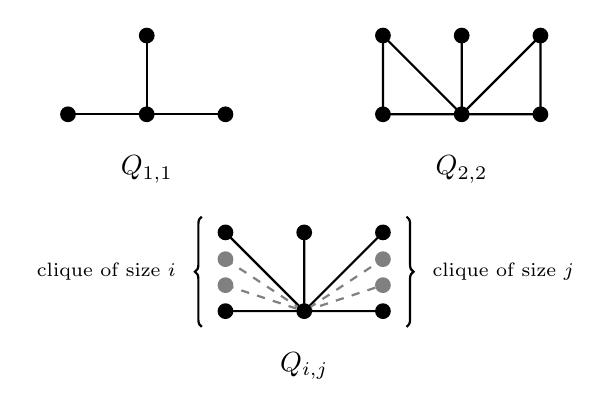
\begin{tikzpicture}[scale=1]

\def\ver{0.1} %size of a vertex
\def\x{1}

\def\xa{0}
\def\ya{0}

\def\xb{4}
\def\yb{0}

\def\xc{9}
\def\yc{0}

\def\xd{2}
\def\yd{-2.5}

\path[fill] (\xa,\ya) circle (\ver);
\path[fill] (\xa,\ya+1) circle (\ver);
\path[fill] (\xa+1,\ya) circle (\ver);
\path[fill] (\xa-1,\ya) circle (\ver);

\draw[thick] (\xa-1,\ya)--(\xa+1,\ya) (\xa,\ya) -- (\xa,\ya+1);

\node (1) at (\xa,\ya-0.7) {$Q_{1,1}$};


\path[fill] (\xb,\yb) circle (\ver);
\path[fill] (\xb,\yb+1) circle (\ver);
\path[fill] (\xb+1,\yb) circle (\ver);
\path[fill] (\xb+1,\yb+1) circle (\ver);
\path[fill] (\xb-1,\yb) circle (\ver);
\path[fill] (\xb-1,\yb+1) circle (\ver);

\draw[thick] (\xb-1,\yb)--(\xb+1,\yb)
(\xb,\yb) -- (\xb,\yb+1)
(\xb-1,\yb) -- (\xb-1,\yb+1) -- (\xb,\yb) -- (\xb+1,\yb+1) -- (\xb+1,\yb);

\node (1) at (\xb,\yb-0.7) {$Q_{2,2}$};


\draw[thick] (\xd-1,\yd)--(\xd+1,\yd)
(\xd,\yd) -- (\xd,\yd+1)
(\xd-1,\yd+1) -- (\xd,\yd) -- (\xd+1,\yd+1);
\draw[thick, dashed, color=gray] (\xd-1,\yd+.33) -- (\xd,\yd) -- (\xd+1,\yd+.33);
\draw[thick, dashed, color=gray] (\xd-1,\yd+.66) -- (\xd,\yd) -- (\xd+1,\yd+.66);

\path[fill] (\xd,\yd) circle (\ver);
\path[fill] (\xd,\yd+1) circle (\ver);
\path[fill] (\xd+1,\yd) circle (\ver);
\path[fill=gray] (\xd+1,\yd+0.33) circle (\ver);
\path[fill=gray] (\xd+1,\yd+0.66) circle (\ver);
\path[fill] (\xd+1,\yd+1) circle (\ver);
\path[fill] (\xd-1,\yd) circle (\ver);
\path[fill=gray] (\xd-1,\yd+.33) circle (\ver);
\path[fill=gray] (\xd-1,\yd+.66) circle (\ver);
\path[fill] (\xd-1,\yd+1) circle (\ver);

%\draw (\xd-1,\yd+0.5) ellipse (0.5 and 1);
%\draw (\xd+1,\yd+0.5) ellipse (0.5 and 1);

\draw[thick,decoration={brace,mirror,raise=0.2cm},decorate] (\xd+1.1,\yd-.2) -- (\xd+1.1,\yd+1.2)
node [pos=0.5,anchor=west,xshift=+0.4cm] {\scriptsize clique of size $j$};
\draw[thick,decoration={brace,mirror,raise=0.2cm},decorate] (\xd-1.1,\yd+1.2) -- (\xd-1.1,\yd-.2)
node [pos=0.5,anchor=east,xshift=-0.4cm] {\scriptsize clique of size $i$};

\node (1) at (\xd,\yd-0.7) {$Q_{i,j}$};


\end{tikzpicture}
\end{center}
\caption{The family of graphs $\mathcal{Q}$.}\label{fig:graph_Q}
\end{figure}

\begin{claim}\label{claim:graph_Q}
  The family of graphs $\mathcal{Q}$ is a subset of the class of thin strip graphs and can be realized such that the position of every vertex is different.
\end{claim}

\proof{
We proceed to realize $Q_{1,1}$ and $Q_{2,2}$ as thin strip graphs. With their realizations we can also deduce the realization of $Q_{i,j}$ for every $i,j \in \mathbb{N}_0$. The clique of size $i$ is called $A$ and the clique of size $j$ is called $B$ based on Figure \ref{fig:graph_Q}.

$Q_{1,1}$ is $K_{1,3}$ and it has been shown that it is realizable as a thin strip graph with coordinates $(0,0), (-1,0), (1,0), (0,\varepsilon)$ for $\varepsilon > 0$. We can realize $Q_{i,j}$ if the position of every vertex in $A$ equals $(-1,0)$ and $(1,0)$ for $B$. However, we want that every vertex of $A$ and $B$ has a different position, so we proceed to construct a realization that holds for $Q_{2,2}$.

Let $a,b,c,d$ be the vertices of a graph $K_{1,3}$ where $c$ is the vertex of highest degree. $a$ and $b$ are the leftmost and rightmost vertices when realized as a thin strip graph, so their positions are $(-1,0)$ and $(1,0)$ respectively and $c$ is the top disk with coordinates $(0, \varepsilon)$ as seen in Figure \ref{fig:graph_Q_real}. If we add now the vertices $e$ and $f$ with the same neighbourhood as $a$ and $b$, we have to find out how much they can move with respect to $a$ and $b$ to still be in contact with $d$ and not with $c$. We can build this new position by taking the same $y$-coordinate as $a$ and $b$, so for the moment $\phi_y(e) = 0$ and $\phi_y(f) = 0$. We can see that the procedure is the same for $e$ and $f$ by symmetry, so we are going to prove this for $e$.

If $\phi_y(e)=0$, then we have to find $\phi_x(e)$ such that $e$ is not in contact with $c$ with a position $\phi(c) = (0, \varepsilon)$.

\begin{equation*}
  \begin{split}
    \sqrt{\phi_x(e)^2 + \varepsilon^2} &> 1\\
    \phi_x(e)^2 + \varepsilon^2 &> 1\\
    \phi_x(e)^2 &> 1 - \varepsilon^2\\
    \phi_x(e) &> \sqrt{1 - \varepsilon^2}\ \ \text{or}\ \  \phi_x(e) < -\sqrt{1 - \varepsilon^2}
  \end{split}
\end{equation*}

with $\varepsilon > 0$.

With this, we can see that $\phi_x(e) \in (-1, -\sqrt{1 - \varepsilon^2})$ and $\phi_x(f) \in (\sqrt{1 - \varepsilon^2},1)$. To finalize this proof, we can see that every vertex of $v \in A$ such that $\phi_x(v)\in (-1, -\sqrt{1 - \varepsilon^2})$, we have infinitely different positions to choose. The same holds for $B$. \qed
}

\begin{figure}[t]
\begin{center}
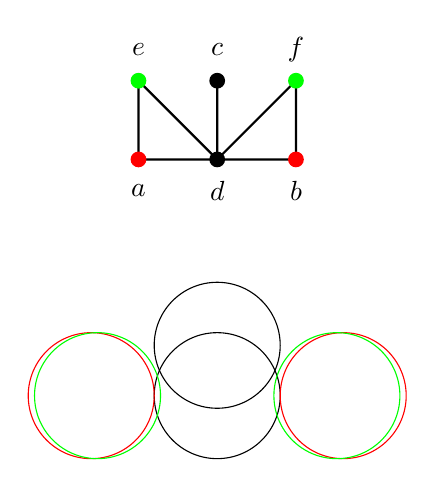
\begin{tikzpicture}[scale=1]

\def\ver{0.1} %size of a vertex
\def\verc{0.8}

\def\x{1}

\def\xa{0}
\def\ya{0}

\def\xb{4}
\def\yb{0}

\def\xd{\xb}
\def\yd{-3}


\draw[thick] (\xb-1,\yb)--(\xb+1,\yb)
(\xb,\yb) -- (\xb,\yb+1)
(\xb-1,\yb) -- (\xb-1,\yb+1) -- (\xb,\yb) -- (\xb+1,\yb+1) -- (\xb+1,\yb);

\node (1) at (\xb,\yb-0.4) {$d$};
\node (1) at (\xb,\yb+1.4) {$c$};
\node (1) at (\xb+1,\yb-0.4) {$b$};
\node (1) at (\xb+1,\yb+1.4) {$f$};
\node (1) at (\xb-1,\yb-0.4) {$a$};
\node (1) at (\xb-1,\yb+1.4) {$e$};

\path[fill] (\xb,\yb) circle (\ver);
\path[fill] (\xb,\yb+1) circle (\ver);
\path[fill=red] (\xb+1,\yb) circle (\ver);
\path[fill=green] (\xb+1,\yb+1) circle (\ver);
\path[fill=red] (\xb-1,\yb) circle (\ver);
\path[fill=green] (\xb-1,\yb+1) circle (\ver);



\draw (\xd,\yd) circle (\verc);
\draw (\xd,\yd+0.4*\verc*2) circle (\verc);
\draw[color=red] (\xd-\verc*2,\yd) circle (\verc);
\draw[color=red] (\xd+\verc*2,\yd) circle (\verc);
\draw[color=green] (\xd-0.95*\verc*2,\yd) circle (\verc);
\draw[color=green] (\xd+0.95*\verc*2,\yd) circle (\verc);

\end{tikzpicture}
\end{center}
\caption{The graph $Q_{2,2}$ and its realization. You can see that the green disk is shifted towards the center with respect to the red one and still does not touch the top disk.}\label{fig:graph_Q_real}
\end{figure}

With this result, we proceed to show the realization of $\mathcal{T}$, $\mathcal{S}$ and $\mathcal{S''}$ as thin strip graphs.


\begin{figure}
\begin{center}
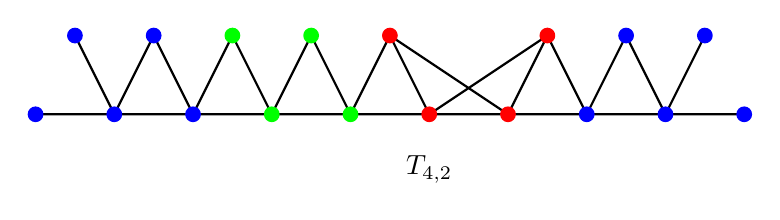
\begin{tikzpicture}[scale=1]
\def\ver{0.1} %size of a vertex
\def\x{1}

\def\xa{0}
\def\ya{0}

\def\xb{4}
\def\yb{0}

\def\xc{9}
\def\yc{0}

\def\xd{3}
\def\yd{-2.5}

\draw[thick] (\xc-2,\yc)--(\xc+7,\yc)
(\xc-1.5,\yc+1)--(\xc-1,\yc)--(\xc-0.5,\yc+1)--(\xc,\yc)--(\xc+0.5,\yc+1)--(\xc+1,\yc)--(\xc+1.5,\yc+1)--(\xc+2,\yc)--(\xc+2.5,\yc+1)--(\xc+3,\yc)--(\xc+4.5,\yc+1)
(\xc+5.5,\yc+1)--(\xc+5,\yc)--(\xc+4.5,\yc+1)--(\xc+4,\yc)--(\xc+2.5,\yc+1)
(\xc+5.5,\yc+1)--(\xc+6,\yc)--(\xc+6.5,\yc+1);

%graph T_{2,1}
\path[fill=blue] (\xc-2,\yc) circle (\ver);
\path[fill=blue] (\xc-1,\yc) circle (\ver);
\path[fill=blue] (\xc,\yc) circle (\ver);
\path[fill=green] (\xc+1,\yc) circle (\ver);
\path[fill=green] (\xc+2,\yc) circle (\ver);
\path[fill=red] (\xc+3,\yc) circle (\ver);
\path[fill=red] (\xc+4,\yc) circle (\ver);
\path[fill=blue] (\xc+5,\yc) circle (\ver);
\path[fill=blue] (\xc+6,\yc) circle (\ver);
\path[fill=blue] (\xc+7,\yc) circle (\ver);

\path[fill=blue] (\xc-1.5,\yc+1) circle (\ver);
\path[fill=blue] (\xc-0.5,\yc+1) circle (\ver);
\path[fill=green] (\xc+0.5,\yc+1) circle (\ver);
\path[fill=green] (\xc+1.5,\yc+1) circle (\ver);
\path[fill=red] (\xc+2.5,\yc+1) circle (\ver);
\path[fill=red] (\xc+4.5,\yc+1) circle (\ver);
\path[fill=blue] (\xc+5.5,\yc+1) circle (\ver);
\path[fill=blue] (\xc+6.5,\yc+1) circle (\ver);

\node (1) at (\xc+3,\yc-0.7) {$T_{4,2}$};

\end{tikzpicture}
\end{center}
\caption{The graph $T_{4,2}$ with the diamond in red and the arms in green. The $Q_{2,1}$ from previous lemma are in blue.}\label{fig:graph_T_clique}
\end{figure}

\begin{figure}[b]
\begin{center}
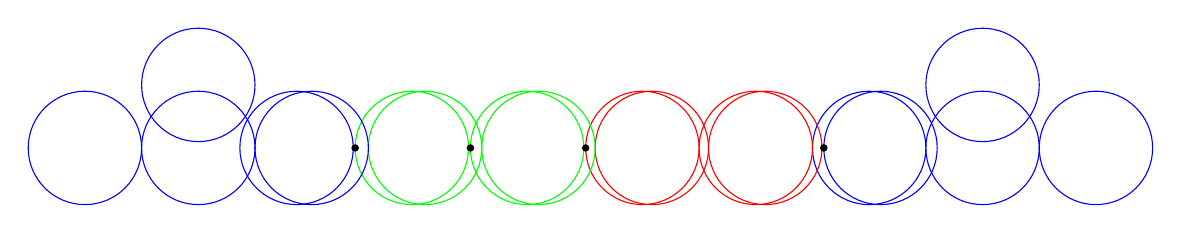
\begin{tikzpicture}[rotate=0, scale=1.2]

\def\ver{0.6}
\def\verp{0.04} %size of a vertex

\draw[color=blue] (\ver*4-0.1,0) circle (\ver);
\draw[color=blue] (\ver*4-0.1+0.12,0) circle (\ver);
\draw[color=blue] (\ver*6-0.1,0) circle (\ver);
\draw[color=blue] (\ver*6-0.1,\ver+\ver/9) circle (\ver);
\draw[color=blue] (\ver*8-0.1,0) circle (\ver);

\draw[color=red] (0,0) circle (\ver);
\draw[color=red] (\ver*2-0.1,0) circle (\ver);
\draw[color=red] (\ver*2,0) circle (\ver);
\draw[color=red] (-0.1,0) circle (\ver);
\draw[color=green] (-\ver*2,0) circle (\ver);
\draw[color=green] (-\ver*2-0.12,0) circle (\ver);
\draw[color=green] (-\ver*4,0) circle (\ver);
\draw[color=green] (-\ver*4-0.14,0) circle (\ver);
\draw[color=blue] (-\ver*6,0) circle (\ver);
\draw[color=blue] (-\ver*6-0.16,0) circle (\ver);
\draw[color=blue] (-\ver*8,0) circle (\ver);
\draw[color=blue] (-\ver*8,\ver+\ver/9) circle (\ver);
\draw[color=blue] (-\ver*10,0) circle (\ver);

\path[fill] (\ver*3+0.02,0) circle (\verp);
\path[fill] (-\ver-0.1,0) circle (\verp);
\path[fill] (-\ver*3-0.12,0) circle (\verp);
\path[fill] (-\ver*5-0.14,0) circle (\verp);

\end{tikzpicture}
\end{center}
\caption{A realization as a thin strip graph of $T_{4,2}$ from Figure \ref{fig:graph_T_clique}. The distance between the disks disminishes with the value of $\varepsilon$, but the disks designated by the black points will never touch.}\label{fig:graph_T_realization}
\end{figure}

\begin{theorem}\label{theo:T_TSG}
  $\mathcal{T}$ is a family of thin strip graphs.
\end{theorem}

\proof{
We take as a reference $T_{4,2}$ in Figure \ref{fig:graph_T_clique}. We can partition this graph in three parts: the \emph{hands} (blue), the \emph{arms} (green) and the \emph{diamond} in the center (red). You may notice that the "hands" are actually $Q_{2,1}$ from Claim \ref{claim:graph_Q}. We begin placing the left "hand" by minimizing the $x$-coordinate of the fifth node as stated in the claim, we give it a $x$-coordinate with value:

$$\tau_0 = \sqrt{1 - \varepsilon^2} + \delta$$

with $0 < \delta < 1 - \sqrt{1 - \varepsilon^2}$. And its $y$-coordinate equals 0, following the same procedure as in the claim.

Next, we place the disks that represent the "arm" of our graph. We place them by clique levels of two indexed by $i \geqslant 1$ from left to right with respect to Figure \ref{fig:graph_T_clique}. The $y$-coordinate of the entire arm equals $0$, it is actually an unit interval graph. We only have to set the $x$-coordinate of each one of the disks $u_i,v_i$ of our level indexed by $i$. The disk $u_i$ will be placed at the $x$-coordinate $i+1$, it will be adjacent to $u_{i-1}$ or the rightmost vertex of the "hand" if $i = 1$. On the other hand, our second disk $v_i$ will be placed in the $x$-coordinate:

$$\tau_i = \tau_{i-1} + 1 + \delta$$

with $0 < \delta < i - \tau_{i-1}$ so that $v_i$ will be on the left of $u_i$. We do this consecutively for each level until we arrive to the diamond. The two leftmost vertices of the diamond are built as a level of the "arm". However, the right two vertices have the same coordinates of the left ones but shifted by one on the $x$-coordinate. By symmetry, the right arm is built equally, by taking care that the last level corresponds with the coordinates of the diamond. You can find the realization of $T_{4,2}$ as a thin strip graph in Figure \ref{fig:graph_T_realization}.
}

This proof will be used as a basis that we are going to use to construct the realization of $\mathcal{S}$ and $\mathcal{S''}$ because as you can see, their structure is very similar. Actually, the "hand" and "arm" that have been used during the proof are directly applicable for the other graphs.

\begin{figure}
\begin{center}
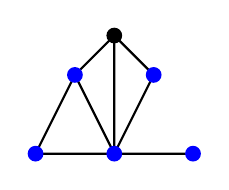
\begin{tikzpicture}[scale=1]
\def\ver{0.1} %size of a vertex
\def\x{1}

\def\xa{0}
\def\ya{0}

\def\xb{4}
\def\yb{0}

\def\xc{9}
\def\yc{0}

\def\xd{3}
\def\yd{-2.5}

\draw[thick] (\xb+1,\yb)--(\xb+2,\yb)--(\xb+3,\yb)
(\xb+1,\yb)--(\xb+1.5,\yb+1)--(\xb+2,\yb)--(\xb+2.5,\yb+1)
--(\xb+2,\yb+1.5)--(\xb+2,\yb)
(\xb+1.5,\yb+1)--(\xb+2,\yb+1.5);


%graph S_1
\path[fill=blue] (\xb+1,\yb) circle (\ver);
\path[fill=blue] (\xb+2,\yb) circle (\ver);
\path[fill=blue] (\xb+3,\yb) circle (\ver);
\path[fill] (\xb+2,\yb+1.5) circle (\ver);
\path[fill=blue] (\xb+1.5,\yb+1) circle (\ver);
\path[fill=blue] (\xb+2.5,\yb+1) circle (\ver);


\end{tikzpicture}
\end{center}
\caption{The graph $S_{1}$. We have colored the induced $Q_{1,2}$ in blue.}\label{fig:graph_S1_clique}
\end{figure}

\begin{figure}
\begin{center}
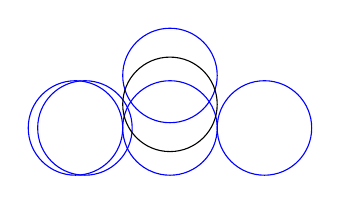
\begin{tikzpicture}[scale=1]
\def\ver{0.6} %size of a vertex
\def\x{1}

\def\xa{0}
\def\ya{0}

\def\xb{4}
\def\yb{0}

\def\xc{9}
\def\yc{0}

\def\xd{3}
\def\yd{-2.5}

\draw[color=blue] (\ver*4-0.1,0) circle (\ver);
\draw[color=blue] (\ver*4-0.1+0.12,0) circle (\ver);
\draw[color=blue] (\ver*6-0.1,0) circle (\ver);
\draw[color=blue] (\ver*6-0.1,\ver+\ver/9) circle (\ver);
\draw (\ver*6-0.1,\ver-\ver/2) circle (\ver);
\draw[color=blue] (\ver*8-0.1,0) circle (\ver);

\end{tikzpicture}
\end{center}
\caption{A realization of $S_1$ as a thin strip graph.}\label{fig:graph_S1_realization}
\end{figure}


\begin{figure}
\begin{center}
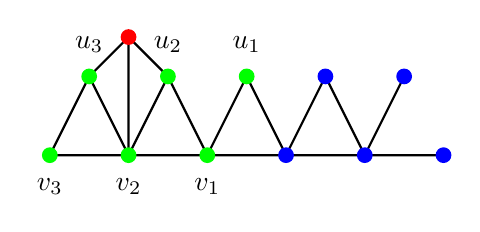
\begin{tikzpicture}[scale=1]
\def\ver{0.1} %size of a vertex
\def\x{1}

\def\xa{0}
\def\ya{0}

\def\xb{4}
\def\yb{0}

\def\xc{9}
\def\yc{0}

\def\xd{3}
\def\yd{-2.5}


\draw[thick] (\xc,\yc)--(\xc+5,\yc)
(\xc+0.5,\yc+1)--(\xc+1,\yc)--(\xc+1.5,\yc+1)--(\xc+2,\yc)--(\xc+2.5,\yc+1)--(\xc+3,\yc)--(\xc+3.5,\yc+1)--(\xc+4,\yc)--(\xc+4.5,\yc+1)
(\xc,\yc)--(\xc+0.5,\yc+1)--(\xc+1,\yc+1.5)--(\xc+1.5,\yc+1)
(\xc+1,\yc)--(\xc+1,\yc+1.5);

%graph S_2
\path[fill=green] (\xc,\yc) circle (\ver);
\path[fill=green] (\xc+1,\yc) circle (\ver);
\path[fill=green] (\xc+2,\yc) circle (\ver);
\path[fill=blue] (\xc+3,\yc) circle (\ver);
\path[fill=blue] (\xc+4,\yc) circle (\ver);
\path[fill=blue] (\xc+5,\yc) circle (\ver);
\path[fill=green] (\xc+0.5,\yc+1) circle (\ver);
\path[fill=green] (\xc+1.5,\yc+1) circle (\ver);
\path[fill=green] (\xc+2.5,\yc+1) circle (\ver);
\path[fill=blue] (\xc+3.5,\yc+1) circle (\ver);
\path[fill=blue] (\xc+4.5,\yc+1) circle (\ver);
\path[fill=red] (\xc+1,\yc+1.5) circle (\ver);


\node (1) at (\xc,\yc-0.4) {$v_3$};
\node (1) at (\xc+1,\yc-0.4) {$v_2$};
\node (1) at (\xc+2,\yc-0.4) {$v_1$};

\node (1) at (\xc+.5,\yc+1.4) {$u_3$};
\node (1) at (\xc+1.5,\yc+1.4) {$u_2$};
\node (1) at (\xc+2.5,\yc+1.4) {$u_1$};

\end{tikzpicture}
\end{center}
\caption{The graph $S_{4}$ with the arm in green and the induced $Q_{2,1}$ in blue. We also noted the vertices of each level of the arm.}\label{fig:graph_S4_clique}
\end{figure}

\begin{figure}
\begin{center}
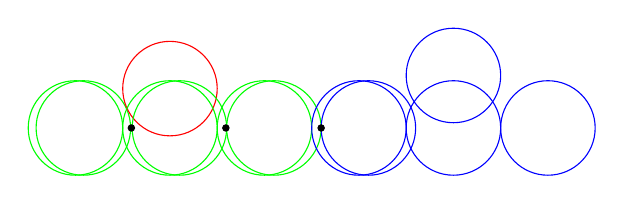
\begin{tikzpicture}[scale=1]
\def\ver{0.6} %size of a vertex
\def\verp{0.04}
\def\x{1}

\def\xa{0}
\def\ya{0}

\def\xb{4}
\def\yb{0}

\def\xc{9}
\def\yc{0}

\def\xd{3}
\def\yd{-2.5}


\draw[color=green] (-\ver*2-0.1,0) circle (\ver);
\draw[color=green] (-\ver*2,0) circle (\ver);
\draw[color=red] (-0.1,0.5) circle (\ver);
\draw[color=green] (-0.1,0) circle (\ver);
\draw[color=green] (-0.1+0.12,0) circle (\ver);
\draw[color=green] (\ver*2-0.1,0) circle (\ver);
\draw[color=green] (\ver*2-0.1+0.12,0) circle (\ver);
\draw[color=blue] (\ver*4-0.1,0) circle (\ver);
\draw[color=blue] (\ver*4-0.1+0.12,0) circle (\ver);
\draw[color=blue] (\ver*6-0.1,0) circle (\ver);
\draw[color=blue] (\ver*6-0.1,\ver+\ver/9) circle (\ver);
\draw[color=blue] (\ver*8-0.1,0) circle (\ver);

\draw[fill] (-\ver+0.01,0) circle (\verp);
\draw[fill] (\ver+0.01,0) circle (\verp);
\draw[fill] (\ver*3+0.02,0) circle (\verp);


\end{tikzpicture}
\end{center}
\caption{A realization of $S_4$ as a thin strip graph based on Figure \ref{fig:graph_S4_clique}. The black points indicate that the disks do not touch at that spot.}\label{fig:graph_S4_realization}
\end{figure}

\begin{theorem}
  \label{theo:S_TSG}
  $\mathcal{S}$ is a family of thin strip graphs.
\end{theorem}

\proof{
In this case, we are going to construct $S_1$ and $S_i$ with $i > 1$ differently. For $S_1$, we build the induced $Q_{2,1}$ as described on \ref{fig:graph_S1_clique}. Then, we add another disk on the center such that its $y$-coordinate is bigger than $0$ and smaller than $\varepsilon$ with a certain value that it touches the left disk as shown in Figure \ref{fig:graph_S1_realization}.

In the other hand, for $S_i$ with $i > 1$ the construction is quite different. Indeed, we can see by Figure \ref{fig:graph_S4_clique} that the "arm" and "hand" subgraphs are exactly the same as for $\mathcal{T}$ in Figure \ref{fig:graph_T_clique}. The same construction works in this case. Now, we only have to add the red vertex $w$ that differs, as seen in \ref{fig:graph_S4_clique}. If we take the same notation as in Theorem \ref{theo:T_TSG}, we construct the arms by clique levels of two vertices of $u_i$ and $v_i$. With this information,
we see that we have an arm of $i-1$ levels in a graph $S_i$ with $i > 1$. The last vertex $w$ can be placed at the $x$-coordinate of $v_{i-2}$ at a $y$-coordinate smaller than $\varepsilon$ so that $w$ is adjacent to $u_3$ and does not touch a vertex from the hand when $i = 2$. You can find the final realization of our example $S_4$ in Figure \ref{fig:graph_S4_clique}. \qed
}

\begin{figure}
\begin{center}
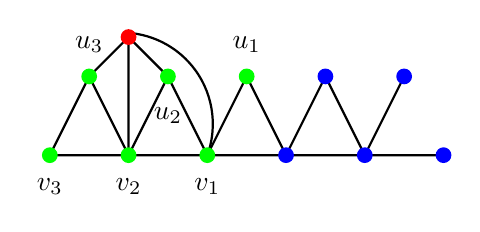
\begin{tikzpicture}[scale=1]
\def\ver{0.1} %size of a vertex
\def\x{1}

\def\xa{0}
\def\ya{0}

\def\xb{4}
\def\yb{0}

\def\xc{9}
\def\yc{0}

\def\xd{3}
\def\yd{-2.5}


\draw[thick] (\xc,\yc)--(\xc+5,\yc)
(\xc+0.5,\yc+1)--(\xc+1,\yc)--(\xc+1.5,\yc+1)--(\xc+2,\yc)--(\xc+2.5,\yc+1)--(\xc+3,\yc)--(\xc+3.5,\yc+1)--(\xc+4,\yc)--(\xc+4.5,\yc+1)
(\xc,\yc)--(\xc+0.5,\yc+1)--(\xc+1,\yc+1.5)--(\xc+1.5,\yc+1)
(\xc+1,\yc)--(\xc+1,\yc+1.5);

\draw[thick] (\xc+2,\yc) arc(-20:85:1.16);

%graph S_2
\path[fill=green] (\xc,\yc) circle (\ver);
\path[fill=green] (\xc+1,\yc) circle (\ver);
\path[fill=green] (\xc+2,\yc) circle (\ver);
\path[fill=blue] (\xc+3,\yc) circle (\ver);
\path[fill=blue] (\xc+4,\yc) circle (\ver);
\path[fill=blue] (\xc+5,\yc) circle (\ver);
\path[fill=green] (\xc+0.5,\yc+1) circle (\ver);
\path[fill=green] (\xc+1.5,\yc+1) circle (\ver);
\path[fill=green] (\xc+2.5,\yc+1) circle (\ver);
\path[fill=blue] (\xc+3.5,\yc+1) circle (\ver);
\path[fill=blue] (\xc+4.5,\yc+1) circle (\ver);
\path[fill=red] (\xc+1,\yc+1.5) circle (\ver);


\node (1) at (\xc,\yc-0.4) {$v_3$};
\node (1) at (\xc+1,\yc-0.4) {$v_2$};
\node (1) at (\xc+2,\yc-0.4) {$v_1$};

\node (1) at (\xc+.5,\yc+1.4) {$u_3$};
\node (1) at (\xc+1.5,\yc+0.5) {$u_2$};
\node (1) at (\xc+2.5,\yc+1.4) {$u_1$};

\end{tikzpicture}
\end{center}
\caption{The graph $S_{4}''$ with the arm in green and the induced $Q_{2,1}$ in blue. We also noted the vertices of each level of the arm.}\label{fig:graph_S24_clique}
\end{figure}

\begin{figure}
\begin{center}
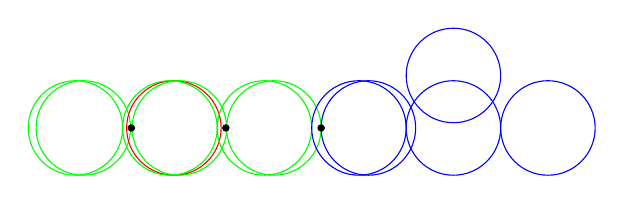
\begin{tikzpicture}[scale=1]
\def\ver{0.6} %size of a vertex
\def\verp{0.04}
\def\x{1}

\def\xa{0}
\def\ya{0}

\def\xb{4}
\def\yb{0}

\def\xc{9}
\def\yc{0}

\def\xd{3}
\def\yd{-2.5}


\draw[color=green] (-\ver*2-0.1,0) circle (\ver);
\draw[color=green] (-\ver*2,0) circle (\ver);
\draw[color=red] (-0.05,0) circle (\ver);
\draw[color=green] (-0.1,0) circle (\ver);
\draw[color=green] (-0.1+0.12,0) circle (\ver);
\draw[color=green] (\ver*2-0.1,0) circle (\ver);
\draw[color=green] (\ver*2-0.1+0.12,0) circle (\ver);
\draw[color=blue] (\ver*4-0.1,0) circle (\ver);
\draw[color=blue] (\ver*4-0.1+0.12,0) circle (\ver);
\draw[color=blue] (\ver*6-0.1,0) circle (\ver);
\draw[color=blue] (\ver*6-0.1,\ver+\ver/9) circle (\ver);
\draw[color=blue] (\ver*8-0.1,0) circle (\ver);

\draw[fill] (-\ver+0.01,0) circle (\verp);
\draw[fill] (\ver+0.01,0) circle (\verp);
\draw[fill] (\ver*3+0.02,0) circle (\verp);


\end{tikzpicture}
\end{center}
\caption{A realization of $S_4''$ as a thin strip graph based on Figure \ref{fig:graph_S24_clique}. The black points indicate that the disks do not touch at that spot.}\label{fig:graph_S24_realization}
\end{figure}

\begin{theorem}
  $\mathcal{S''}$ is a family of thin strip graphs.
\end{theorem}

\proof{
This family of graphs is a variant of $\mathcal{S}$ and as proven on Theorem \ref{theo:S_TSG} it is a subset of TSG. The only difference here is that now the red vertex $w$ is also adjacent to $v_1$. In this case, we can simply place $w$ at the $y$-coordinate $0$ like the other vertices of the arm. The $x$-coordinate can be any position between the $x$-coordinates of $v_2$ and $v_1$. A realization can be found in \ref{fig:graph_S24_realization}.
}

Now we have a slightly better understanding of the structure of TSG. We have proven in this section that $\mathcal{R}$ is the only family of forbidden subgraphs of MUIG that is also forbidden for TSG. Moreover, $\mathcal{R}$ is also forbidden for UUIG. A good starting point, as stated by Hayashi \textit{et al.} \cite{hayashiThinStripGraphs2017}, is to find a graph that is in $(\text{UDG} \cap \text{UUIG}) \setminus \text{TSG}$. This graph will be the key for understanding what are the graph structures that are not likely to be a TSG.


\section{Recognition}

The recognition of this class of graphs is approached by Breu in his thesis \cite{breuAlgorithmicAspectsConstrained1996}. He gives a polynomial-time algorithm to recognise strip graphs for a given input with an assignment of $y$-coordinates for each vertex of the graph and an orientation of the edges of its complement.

\begin{theorem}[Breu \cite{breuAlgorithmicAspectsConstrained1996}]
  Let $G = (V,E,\gamma,\overrightarrow{E})$ a graph where $\gamma: V \to [0,c]$ is a function associating a $y$-coordinate (or a level) to each vertex and $\overrightarrow{E}$ an orientation of the complement of the graph. The recognition of $c$-strip graphs with this input is in $\mathcal{P}$.
\end{theorem}

\begin{obs}
  Recognition of $c$-strip graphs without a given $\overrightarrow{E}$ is in $\mathcal{NP}$.
\end{obs}

\proof{
  Given a polynomial-time algorithm with a complexity of $\mathcal{O}(f(n))$ to solve recognition of $G = (V,E,\gamma,\overrightarrow{E})$, we can run again this algorithm by testing every possible orientation of its complement. This algorithm would take $\mathcal{O}(f(n))2^{|E|-1} = \mathcal{O}(f(n)2^{|E|})$ time to execute. \qed
}\\

We would like to have an algorithm that solves this problem without knowing the $y$-coordinates of the vertices. Nevertheless, further research would concentrate on recognition of UUIGs. We know that TSG $\subsetneq$ UUIG, and recognition of UUIGs is $\mathcal{NP}$. If we the problem of recognising TSG given a UUIG and is solved in polynomial time, then TSG recognition would be $\mathcal{NP}$. However, given the observations in the end of chapter \ref{chap:interval}, there may be a polynomial-time algorithm for UUIG.
